% This file is responsible to collect all content and assemble the document.

% Edit these lines...
\def\thesisType{Master Thesis}
\def\name{HAKKEL Tamás}
\def\program{Computer Science Engineering MSc}
\def\title{Iteratively Reweighted Algorithms for Dynamic MRI}
\def\supervisors{Supervisor: Claudio M. VERDUN \\ Faculty mentor: Dr. OLÁH András}

% ---------------------------------------------

% Render title page
\titlePage

% Set page numbering to roman numbers for all pages before the first chapter. Change it to "\pagenumbering{Roman}" if you want upper case roman numbers
\pagenumbering{roman}

% Mandatory parts
% If you don't want these mandatory parts to be included in the table of contents, simply delete or comment out the lines starting with "\addcontentsline".
\addcontentsline{toc}{chapter}{Diploma Thesis Proposal}

% If you print your thesis two sided, the you need this blank page after the Title page
\blankPage

% The "Diploma Thesis Proposal" form takes the first two page numbers, so the "Thesis Authenticity Statement" gets the page number 3.
\setcounter{page}{3}

\addcontentsline{toc}{chapter}{Thesis Authenticity Statement}
% You have nothing to do here

\chapter*{Thesis Authenticity Statement}
I, undersigned \name, student of the Faculty of Information Technology and Bionics at the Pázmány Péter Catholic University, hereby certify that this thesis was written without any unauthorized help, solely by me and I used only the referenced sources. Every part, which is quoted exactly or in a paraphrased manner, is indicated clearly with a reference. I have not submitted this thesis anywhere else.

% Signature line
\begin{flushright}
	\vspace*{.5cm}\par\noindent\makebox[2.5in]{\hrulefill}
	\par\noindent\makebox[2.5in][c]{\name}
\end{flushright}

\clearpage
\addcontentsline{toc}{chapter}{Abstract}
\chapter*{Abstract}

Although MR imagig was invented less then 50 years ago, it has revolutionized medical imaging and diagnostic process as we know it. Its versatility makes it fit a wide range of use cases, and compared to other imaging technologies, MRI demonstrates important advantages in many cases, such as lack of ionizing radiation, adjustable contrast range, and excellent differentiation between soft tissues. However, it has also a disadvantage: the imaging speed is undesirably slow. While it is only inconvenience in some cases, dynamic images of chest, for example, gets blurred by the different motions of the body, like breathing and cardiac motion. There are new technologies that improves the imaging process itself, but strong image reconstruction algorithms can vastly improve the quality.

Among the many software techniques invented to improve image quality, compressed sensing is inevitably is one of the most impactful theoretical construction, introduced by Donoho, Candès, Romberg, and Tao in 2004~\cite{candes_robust_2006, donoho_compressed_2006, candes_nearoptimal_2006}. In contrast to the Nyquist-Shannon theorem that asserts that continuous band-limited signals can be perfectly reconstructed from samples taken at a rate of twice the highest frequency present in the signal of interest, compressed sensing allows lossless reconstruction from much lower number of samples given that certain natural conditions are satisfied.

In this thesis work, we consider the classic results as well as the recent advances within of the compressed sensing framework and their application to real life MR imaging. In particular, we closely examine two recent publications presenting state-of-the-art solutions combining conventional techniques with novel ideas.

Afterwards, we present our implementation of these algorithms along with the implementation of a recently invented algorithm from the family of iteratively reweighted least squares (IRLS) methods that previously have not been applied to MRI setting yet. For the language of implementation we have chosen Julia, a new open-source language released in 2012, as this language fits well the image reconstruction problem being inherently fast with a speed often comparable to C, and providing convenient environment for fast prototyping.

Finally, we compare these algorithm with respect to reconstruction power from massively undersampled data and noise tolerance. Our results demonstrates the fitness of the Julia language to prototyping and also shows strong benchmark suggesting that a robust extension of the new IRLS method can bring enormous improvement to reconstruction quality or imaging speed.

\clearpage
% Uncomment the following line if you want to include an "Acknowledgements" page after the abstract.
%\addcontentsline{toc}{chapter}{Acknowledgements}
%\chapter*{Acknowledgements}
% Optional part to give thanks to people contributing to your work (other than your supervisor and mentor) https://seleninevcilikhayati.com/accounting-dissertation-help/

\paragraph{}
\lipsum[2] % 1 paragraph of dummy text - replace it with your thanksgiving lines
\clearpage

% Render table of contents
\tableofcontents
\clearpage

% From here page numbers are arabic numbers starting again from 1
\pagenumbering{arabic}

% Include files holding the content of your thesis -- feel free to change as you like it
\chapter{Introduction}\label{chapter:introduction}

While the fast evolution of technology profoundly changed today's medicine, unarguably the medical imaging is of the fields which profited the most of the computation power recently became available. And as X-rays revolutionized medical treatments in the beginning of the 20th century, after its discovery by Wilhelm Conrad Röntgen,  the appearance of computer-aided imaging techniques such as computer tomography (CT), diagnostic ultrasonography, positron emission tomography (PET), and magnetic resonance imaging (MRI) opened a new horizon drastically increasing the resolution, allowing 3D imaging, providing reliable dynamic recordings, and enhancing images by automated post-processing \cite{mri_picturetoproton}. In the recent decades radiology evolved to be an interdisciplinary field involving, for instance, molecular biology, nuclear physics, applied mathematics, and computer science besides the classical medical fields such as anatomy, angiology, and cardiology.

\section{Magnetic Resonance Imaging}

In particular, MRI has revolutionized medical imaging and diagnostic process as we know it. Its versatility makes it fit a wide range of use cases. Compared to other imaging technologies, MRI demonstrates important advantages in many cases.
\begin{itemize}
    \item In contrast to X-ray, MRI doesn't use any ionizing radiation, and hence it is totally harmless to the patient. Also, MRI has enhanced resolution for soft tissues compared to any other modality, in particular neural tissue,  while X-rays are rather used for diagnosing bone degeneration, dislocation, fracture or some tissue infection. Furthermore, MRI allows 3D scans. Nevertheless, MRI scanners are slow and expensive compare to X-ray scan machines and therefore hardware and software improvements are necessary for its wider use.
    \item As CT scanning is based on X-rays, it shares the downside with X-rays, doctors need to evaluate the possible benefits of the scan and decide if it outweighs the potential complications of exposure to ionizing radiations. MRI, however, elicit this problem, although at the price of a elongated imaging process. Comparing the medical problems where these technologies are used, one can conclude that CT scan is very helpful in diagnosing severe injuries of the chest, head, spine or abdomen, particularly fractures, and it is commonly used to localize tumors. MRI often performs better at diagnosing problems in the joints, soft tissues, ligaments and tendons. When available, doctors use it frequently to scan the spine, brain, muscles, neck, breasts, and abdomen.
    \item MRI still does not have the portability, low cost, and real-time imaging speed without any harmful radiation of ultrasound technology, but ultrasound is mostly limited to 2D imaging (although 3D imaging is possible), have trouble penetrating bone, and even in absence of bone the depth of penetration is limited depending on the frequency of imaging. This is not the case for MRI technology.
    \item PET scans are particularly useful for functional imaging. For instance, it is used for identification of lapses in cognitive function, examination of cardiac failures, cancer screening and diagnosis, and finding an infection.  Nevertheless, PET image acquisition is even longer than MRI (especially, if we consider also the time while patients wait for the tracer to reach the targeted organ), it uses a radioactive substance as tracer, and it cannot scan tissues not absorbing the tracer making the localization of the source of the signal infeasible without any additional information. In order to solve the latter described limitation, one particularly promising combination is the join use of PET and MRI. This illustrates that MRI is a fundamental technology not only by itself but also when combined with other imaging modalities.
\end{itemize}
To sum up, MRI is a strong competitor to other imaging technologies, but it also have weaknesses, of which the costs and scanning time are the most remarkable. There are many methods to speed up measurements as it will be discussed later, but the construction cost and the hardware constraints limit the applicability of these efforts. The problem of slowness is even more apparent in case of dynamic images as motion of organs (e.g. heart or lung) can drastically degrade the image quality. To overcome that issue, mathematical solutions developed in the last twenty years such as \emph{parallel imaging} and \emph{compressive sensing} made high-resolution and fast images possible. This thesis concerns the second of these two powerful mathematical ideas.

\section{Compressed Sensing}

Among the many software techniques invented to improve image quality, compressed sensing (also known as compressive sensing, compressed sampling, and compressive sampling) is inevitably is one of the most impactful theoretical construction, introduced by Donoho, Candès, Romberg, and Tao in 2004~\cite{candes_robust_2006, donoho_compressed_2006, candes_nearoptimal_2006}. Such importance can be seems by the fact that the four foundational papers of compressive sensing received, at the time of writing this manuscripts, more than 60000 citations. In contrast to the Nyquist-Shannon theorem that asserts that continuous band-limited signals can be perfectly reconstructed from samples taken at a rate of twice the highest frequency present in the signal of interest, compressed sensing allows lossless reconstruction from much lower number of samples given that certain natural conditions are satisfied.

This impressive improvement is due to the same phenomenon that makes modern image compression algorithms so successful: the sparsity of the signal to be recovered in a certain representation domain. And while the classic image processing flow starts with acquiring the fully sampled image, then feeding it to a compression algorithm that discards the vast majority of the data still allowing later a lossless decompression (e.g. JPEG or JPEG2000), the idea behind compressed sensing is that image acquisition can be made much more effective by fusing it with the compression step recording only the data we need later for decompression, hence the name compressed sensing. As will be discussed in this thesis, MRI possess natural sparse representation and due to physics of the nuclear magnetic resonance phenomenon, its acquisition process is dictated by Fourier transforms which makes it a perfect candidate for the use of compressive sensing machinery. Indeed, MRI was the first successful application of compressive sensing \cite{lustig} and, since 2017, MRI scanner employing this technology are approved by the American Food and Drug Administration and commercially available \cite{fda_siemens, fda_GE}.

% THIS SENTENCE WAS WRONG!
% Since MRI scanning operates directly in Fourier domain and all natural images tent to be sparse in the Fourier domain, compressed sensing is particularly effective in accelerating MRI acquisition.

As a trade-off for the acceleration in the scanning time, the posterior process of reconstructing the image from the measured data is much more involved compared to the standard one typically used when longer scans, i.e., fully sampled Fourier measurement, are performed. Therefore, a large amount of theory was developed since the introduction of compressive sensing to further improve the recovery of a high resolution image from the compressed representation. Ideas coming from high-dimensional statistics, non-linear optimization, harmonic analysis and signal processing came together in order to develop robust, stable and scalable reconstruction methods for compressive sensing. These ideas are particularly useful when applied to the MRI field since the minimization problems with its associated cost functions associated tend to be very challenging. Here, a few of those modern ideas will be discussed, in particular, \emph{accelerated proximal methods} and \emph{iteratively reweighted least squares}

% number of studies investigates the possible solutions for the recovery of a high resolution image from the compressed representation. Most of these attempts starts from an already existing optimization method, defines a cost function which is hoped to lead to a more optimal solution, and maybe combines the resulted algorithm with some extra steps helping faster convergence or more exact recovery. But at the same time, new optimization algorithms or variants of existing algorithms are developed continuously, so another way to approach the problem is to try out new algorithms within the conventional frameworks.

\section{Julia Language}
\subsection{Objectives of The Language}
\subsection{Suitability to Our Task}

\section{Objective}

% ----------------------------------------------------
\section{Outline}
The summary of the chapters of the thesis work:

\paragraph{Chapter 2} This chapter describes something and here I summarize it in a couple sentences.

\paragraph{Chapter 3} This chapter describes something and here I summarize it in a couple sentences.

\paragraph{Chapter 4} This chapter describes something and here I summarize it in a couple sentences.

\paragraph{Chapter 5} This chapter describes something and here I summarize it in a couple sentences.

\clearpage % You need \clearpage at the end of every chapter to force images included in this chapter to be rendered in somewhere else
\chapter{Theoretical Background}

\section{Physics of MRI}
\subsection{Components of MRI machines}
The theory of measurements based on nuclear magnetic resonance has its root in quantum physics: The nuclear magnetic moment and the angular momentum of protons in the atomic nuclei maintained by the spin of these particles are to be indirectly measured, and these observables depend (besides many other factors) on the tissue where the proton is located. More specifically, the MRI
machines are tuned to focus on the nucleus of protons that consist of only one proton. The core components of MRI machines are the following:
\begin{enumerate}
    \item Superconductive coils immersed in liquid helium responsible for producing a almost perfectly homogeneous and static magnetic field. The role of the liquid helium is to keep the wires at superconducting temperature, so that massive amounts of electricity can be run through the coils creating super-strong fields up to \SI{21.1}{\tesla}~\cite{schepkin_vivo_2012}. Although stronger magnetic field allows better resolution, the construction costs of such machines and the effect of the strong magnetic field on human tissues limit the strength of available MRI scanners for routine clinical from \SI{0.2}{\tesla} to \SI{3.0}{\tesla}, and up to \SI{11.7}{\tesla} in research machines for human imaging~\cite{ladd_pros_2018}.
    \item Inside of this super-strong electromagnet, the so called gradient coils are located that alter the field along all three dimensions creating spatially varying magnetic field (hence the name: gradient coils) in order of \SI{}{\milli\tesla}, so that signals coming from different location within the coils are possible to be separated. They are also used to provide contrast for diffusion and flow imaging.
    \item Within the Radio Frequency (RF) coils are located that emit and measure time varying electromagnetic signals on order of tens of \SI{}{\micro\tesla}.
\end{enumerate}
The reason behind this elaborate design (depicted on fig.~\ref{fig:mri_schematic}) is the need of creating a measurement setup suitable to give a very fine control over the the direction of the magnetic moment of protons of hydrogen atoms within the measured object (which, in our case, is the human body that contains a large amount of hydrogen mostly in the form of water, but also bounded within other molecules).

\subsection{Macroscopic Magnetization}
The purpose of the superconductive coils is to align the magnetic moment of protons with the direction of the magnetic field. This direction (also corresponding to the head-to-foot direction) is usually referred as longitudinal direction or z direction, and the plane perpendicular to this direction is called the transverse plane or the x-y plane. This alignment of the magnetic moment of the protons leads to two configurations: protons with their magnetic moment pointing to the same direction as the static magnetic field, and other protons having their magnetic moment with opposite direction. Without the static field, the randomly oriented spins cancel out each other, as they also do in the aligned case, when the number of protons oriented to the two directions are equal. But in real systems, a slight excess of the protons aligned with the static magnetic field always produces a net magnetization with the same direction as the external magnetic field.

The ratio of the number of protons in these two groups are described by the Fermi-Dirac statistics. In strong and static magnetic field at room temperature, the Fermi-Dirac distribution reduces to Boltzmann distribution resulting the following formula:
\[N_+ = N \cdot \frac{e^{E_+ / (k_B T)}}{e^{E_+ / (k_B T)} + e^{E_- / (k_B T)}} \text{ and } N_- = N \cdot \frac{e^{E_- / (k_B T)}}{e^{E_+ / (k_B T)} + e^{E_- / (k_B T)}},\]
where $N$ is the total number of protons, $N_+$ and $N_-$ are the numbers of protons pointing to the same and opposite direction as the static magnetic field, $E_+$ and $E_-$ are their respective energy levels, $k_B$ is the Boltzmann-constant, and $T$ is the temperature. In this case neighboring energy levels are equidistant with the difference in the secondary spin quantum number of $\Delta m = \pm 1$ and the energy difference of $\nabla E = \gamma \hbar B_0$, where $\gamma$ is an empirical constant called gyromagnetic ratio (equals to $42.575 \cdot 2\pi$\SI{}{\mega\hertz/\tesla} in case of protons), $\hbar$ is the reduced Planck constant, and $B_0$ is the static external magnetic field. The ratio of Boltzmann distributions for two states a spin \textonehalf nucleus is known as the Boltzmann factor:
\[f(E) = e^{-\frac{\gamma \hbar B_0}{k_B T}}.\]
Using this factor, the ratio of unpaired protons (these protons give the net magnetization) divided by the number of all protons is given by
\[\frac{N_+ - N_-}{N_+ + N_-} = \frac{\gamma \hbar B_0}{2 k_B T}.\]
This ratio at room temperature in a static field with a couple teslas tends to be a tiny number (in the order of \num{1e-6} multiplied by $B_0$), so that explains why do MRI machines need such a strong electromagnets. (Note that this ratio also can be increased by increasing the temperature, but it is not feasible for human imaging.)

\begin{figure}
    \centering
    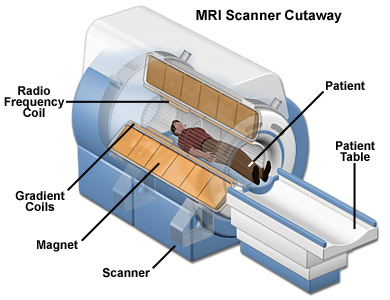
\includegraphics[width=0.45\textwidth]{images/mri-scanner.jpg}
    \caption{Schematic illustration of construction of a cylindrical MRI scanner.\\
    Source: Adapted from~\cite{coyne_mri_2020}}
    \label{fig:mri_schematic}
\end{figure}

\subsection{Precession}
In equilibrium when all protons are aligned with the external magnetic field, the longitudinal component of net magnetization is maximal and the component in the transverse plane is zero. However, with the aid of an electromagnetic excitation in the transverse plane emitted by the RF coils, it is possible to rotate the vector of net magnetization into the transverse plane. The key factor in this process is to tune the frequency of the excitation to match the so called precessional frequency of the protons given by the Larmor equation:
\[\omega = \gamma B_0.\]
The name \textit{precessional frequency} comes from the phenomenon that the magnetic moment of protons start to \textit{precess} around the longitudinal axis (which, again, is the direction of static external magnetic field) due to its intrinsic angular momentum. When the frequency of the excitation matches the precessional frequency of the proton (which happens to be in the radio frequency range, hence the name of RF coils), then resonance occurs and the angle of net magnetization gets tilted, otherwise the electromagnetic field has little to no effect of the net magnetization. An RF excitation of a duration $\tau$ causes rotation of the magnetization by an angle $\theta$, which is called the flip angle, defined by
\[\theta = \gamma \int_0^\tau B_1(t) dt = \gamma \tau B_1,\]
where $B_1$ is the magnetization of RF excitation, and it is assumed to be constant over time window of excitation with length $\tau$.

As a result of the precession, the net magnetic flux changes in the RF coils (these coils used for both emitting and receiving RF signals) inducing an electromotive force $U_{ind}$ that can be calculated by Faraday's law of induction:
\[U_{ind} = -\frac{d\Phi}{dt}.\]
Projecting the precessing movement (with the Larmor frequency $\omega$) of the net magnetization to transversal plan, we get a sinusoidal change in flux that results in the following formula:
\[U_{ind} \sim sin(\theta)\, \omega\, cos(\omega t) = sin(\theta)\, \gamma\, B_0\, cos(\gamma\, B_0\ t).\]
While this formula is not an exact model that fits the current measured in the RF coils, but it captures three important aspects of the resulted electric signal:
\begin{enumerate}
    \item It is a sinusoidal signal with a frequency depending only on a constant specific to protons and the external magnetic field.
    \item The amplitude of that signal depends on the flip angle induced by an RF excitation.
    \item And it is also dependent on the external magnetic field (yet another reason why MRI machines need very strong electromagnets).
\end{enumerate}

\subsection{Relaxation}
For a more accurate model, one should consider that as the protons emit RF signal due to their precessing magnetic moment, they lose the energy of the excitation and they slowly return to the low energy state; i.e., to the state where the magnetic moment of protons are aligned along the longitudinal axis, and where the net magnetization points to the same direction as the external field. Assuming that the excitation resulted in a perpendicular flip angle, the longitudinal component of magnetization is characterized by the exponential formula
\[M_z = M_0 (1 - e^{-t/T_1}),\]
where $M_0$ is the amplitude of magnetization in the equilibrium and is often called Boltzmann magnetization, and $T_1$ time constant is a property of the protons dependent on the tissue where they are located. This process is usually referred as $T_1$ relaxation.

Furthermore, the net magnetization is also affected by another relaxation process referred as $T_2$ relaxation. The phenomenon causing this relaxation is called \textit{dephasing}, and the name comes from the fact that when excitation is applied to protons in the equilibrium, they will precess in the same phase, but soon they lose this synchronization. This desynchronization is due to the slight inhomogeneity of the static external field caused by four factors: spin-spin interactions (quantum mechanical interactions with the nearby protons), magnetic field inhomogeneities (hardware limitations), magnetic susceptibility (slight magnetization of molecules within the measured part of the body), and chemical shift effects (shielding effect of the electron cloud of molecules incorporating the hydrogen atoms). The slightly different $B_0$ value makes the Larmor frequency different, and that results in the desynchronization of phase. The outcome of this process is that the transversal component of the net magnetization decays exponentially to zero. The speed of decay is characterized by the $T_2^*$ time constant:
\[M_{xy} = M_1\,e^{-t/T_2^*},\]
where $M_1$ is the initial amplitude of net magnetization in the beginning of the $T_2$ relaxation process. Using, however, the later described \textit{spin-echo} measurement protocol, the last three inhomogeneity-causing factors can be cancelled out leading to a slightly different time constant denoted by $T_2$.

\subsection{MRI Sequences}
Although the theory explained above are always the same for all MRI measurements, numerous methods exist and are used in today's medicine producing drastically different. These methods are usually referred as MRI sequences and they mostly differ in the a particular setting of RF pulses and the gradients in the static magnetic field, resulting in a particular image appearance. The most commonly used group of MRI sequences is the \textit{spin echo}~\cite{hahn_spin_1950}. In accordance with the two types of relaxation, sequences in that group have two main parameters: $TR$ (Time of Repetition) and $TE$ (Time of Echo). These parameters have a crucial role timing the recording of current in the RF coils when the difference between the amplitude of the RF signal emitted by the excited protons is maximal because this difference makes it possible later to distinguish different tissues.

The $TR$ parameter is connected to the $T_1$ value, as it determines the time between two excitation pulses. Having a larger $TR$ value allows protons to get better aligned with the external magnetic field before the next excitation, which results in a higher initial value for $M_{xy}$, leading to a stronger current in the detector coils, but it also makes the entire measurement longer. On the other hand, $TE$ determines the delay between the peak of the RF pulse and the peak of the echo. That echo is a temporary rephasing of spins caused by a second, \SI{180}{\degree} RF pulse emitted at $t = TE/2$. That pulse inverts spins, and therefore it makes spins with slower Larmor frequency, which lagged behind the faster ones previously, be ahead of the others in phase. At the time when faster precessing protons catch up, the transversal magnetization exhibits an echo peak. As stated earlier, an important advantage of spin echo technique is that three factors of magnetic inhomogeneity is cancelled out by the inversion as these factors are constant over time, while spin-spin interactions are random interactions between protons that cause random local changes in the magnetic fields experienced by the protons.

Based on the choice of $TR$ and $TE$ values, we can talk about three types of spin echo sequences: $T_1$ weighted sequence has intermediate $TR$ value in the magnitude of $T_1$ producing maximal T1 weighting (at this point, the difference caused by different $T_1$ value between the amplitude of signals coming from different tissues are maximal) and short $TE$ value magnitudes smaller than $T_2$ producing minimal T2 weighting (there is not enough time to have significant difference between decay curves with different $T_2$). To the contrary, T2-weighted images have a long $TE$ (maximizing the difference in $T_2$ relaxation) and long $TR$ (reducing the weight of $T_1$ relaxation). And the third type, called proton density (PD) weighting, uses short $TE$ and long $TE$, so that the pixel intensities on the resulted image will reflect only the density of protons (that also differs between tissues), and the $T_1$ and $T_2$ values have little effect on it.

\clearpage
\chapter{Related Works}
% The Code of Studies and Exams recommends the following content for this chapter: "Literature review, short description of similar/related applications/solutions, conclusions of literature review. Independent, critical analysis of the literature."
% However, you are free to structure the content of your thesis as you want

\section{Compressed Sensing in MRI}
"Compressed Sensing MRI" (2008) by Michael Lustig, David L. Donoho, Juan M. Santos, and John M. Pauly --> "A look at how CS can improve on current imaging techniques"

"Sparse MRI: The Application of Compressed Sensing for Rapid MR Imaging" (2007) by Michael Lustig, David Donoho, and John M. Pauly

\section{Parallel Imaging}
"Self-Calibrating Nonlinear Reconstruction Algorithms for Variable Density Sampling and Parallel Reception MRI" by Loubna El Gueddari, C. Lazarus, H Carrié, A. Vignaud, Ph Ciuciu

SENSE and ESPIRiT for sensitivity map estimation

\section{First Order Gradient Methods}

My slideshow about first order methods: \url{https://docs.google.com/presentation/d/1tIZSSfzzHUgo9tlKlmhSUCCWD3ynzyZwnWtpBUe--6g/edit}

\subsection{Origins}
From Cauchy to recent explosion of optimization algorithm.

Why would second order methods speed up convergence and why aren't we able to apply them to our problem.

\subsection{Gradient Descent vs Conjugate Gradient}
How do they work, and when can conjugate gradient outperform gradient descent

\subsection{Proximal Methods and ISTA}
Proximal operator, Iterative Shrinkage/Soft Thresholding Algorithm, Forward-Backward Splitting with linear line search, Wolfe conditions

\subsection{FISTA by Nesterov}
Momentum rule and its role in speeding up convergence

\subsection{POGM by Kim and Fessler}
Why is it faster than FISTA, and why is it optimal

D. Kim and J. A. Fessler, “Optimized first-order methods for smooth convex minimization,” Math. Program., vol. 159, no. 1, pp. 81–107, Sep. 2016, doi: 10.1007/s10107-015-0949-3.

\subsection{ADMM}
what is it and why is it good

\section{Decompositions}

\subsection{Low rank and Sparse}
C. Y. Lin and J. A. Fessler, “Efficient Dynamic Parallel MRI Reconstruction for the Low-Rank Plus Sparse Model,” IEEE Transactions on Computational Imaging, vol. 5, no. 1, pp. 17–26, Mar. 2019, doi: 10.1109/TCI.2018.2882089.

J. A. Fessler, “Optimization methods for MR image reconstruction (long version),” arXiv:1903.03510 [eess, math], Jun. 2019.

\subsection{Multiscale}

Ong's dissertation: “Low Dimensional Methods for High Dimensional Magnetic Resonance Imaging,” 2018.

F. Ong et al., “Extreme MRI: Large-Scale Volumetric Dynamic Imaging from Continuous Non-Gated Acquisitions,” arXiv:1909.13482 [physics], Dec. 2019.

Differences between Ong's dissertation and his "extreme MRI" preprint paper

\section{IRSL}
Iteratively reweighted Least Squares method

C. Kümmerle and C. M. Verdun, “Denoising and Completion of Structured Low-Rank Matrices via Iteratively Reweighted Least Squares,” arXiv:1811.07472 [cs, math], Nov. 2018.

Henry Adams, Lara Kassab, and Deanna Needell "An Iterative Method for Structured Matrix Completion"

\clearpage % You need \clearpage at the end of every chapter to force images included in this chapter to be rendered in somewhere else
\chapter{Implementation details}
% The Code of Studies and Exams recommends the following content for this chapter: "Presentation of used methodologies/technologies: In line with the topic of the dissertation, the professional background related to the solution and implementation of the task must be detailed."
% However, you are free to structure the content of your thesis as you want

\section{FunctionOperators package}
Describe this package what I created, and explain why was it useful.
\subsection{Objective}
\subsection{Features}

\section{Implementation of Sparse+Low Rank algorithms}
Re-implementation of Lin \& Fessler paper
\subsection{PINCAT dataset}
\subsection{Description of Algorithms in the article}

\section{Implementation of Multiscale Decomposition}

\subsection{NUFFT}
\paragraph{What is NUFFT}
\paragraph{Available solutions}
\paragraph{My implementation}

\subsection{Description of algorithm}

\subsection{Optimization possibilities}
\begin{enumerate}
    \item Batch-processing: compute NUFFT of all channels at once
    \item Parallelization:
    \begin{enumerate}
        \item NUFFT
        \item Algorithm
    \end{enumerate}
    \item GPU-specific optimizations:
    \begin{enumerate}
        \item Blocking operator might cause CPU bottleneck
    \end{enumerate}
\end{enumerate}

\subsection{Parallelization Solution}
Details how I made the code run parallel

\section{IRLS Implementation}

\subsection{Description of Algorithm}
\subsection{Implementation Details}

\clearpage % You need \clearpage at the end of every chapter to force images included in this chapter to be rendered in somewhere else

\chapter{Results}
% The Code of Studies and Exams recommends the following content for this chapter: "Evaluation, critical analysis of the implemented technical solutions, possibilities for further development."
% However, you are free to structure the content of your thesis as you want

\section{Sparse + Low Rank Algorithm}
\subsection{Running Speed and Memory Used}
\subsection{Readability}

\section{Multi-scale Algorithm}
\subsection{Running Speed and Memory Used}

\section{ILRS}
\subsection{Comparism with Sparse+Low Rank}
\paragraph{Running speed and memory requirement}
\paragraph{Convergence speed}
\paragraph{Robustness:} Effect of error on the input data
\paragraph{Recovery capability:} Can we reach the same accuracy on recovered image using less data?

\subsection{Comparism with Multi-scale}
\paragraph{Running speed and memory requirement}
\paragraph{Convergence speed}
\paragraph{Robustness:} Effect of error on the input data
\paragraph{Recovery capability:} Can we reach the same accuracy on recovered image using less data?

\clearpage % You need \clearpage at the end of every chapter to force images included in this chapter to be rendered in somewhere else
\chapter{Summary}
% The Code of Studies and Exams recommends the following content for this chapter:
% A summary of the problems solved compared to the objectives presented in the introduction and  in the Thesis Proposal Form. Opportunities to move forward, questions motivating the future works, outlook.
% However, you are free to structure the content of your thesis as you want

\section{Objectives}
\section{Achievements}
\section{Future Plans}

% Bibliography
\printbibliography
\addcontentsline{toc}{chapter}{Bibliography}

% Appendices -- if you don't have any, just delete the following two lines
%\appendix
%\chapter{Appendix}

Here you can present all the materials that helps the understanding of your work, but either 1) not your work, 2) not necessary to understanding, 3) simply just interesting things not directly related to your topic, or 4) your text already exceeded 120 pages, and need to make it shorter by moving parts to appendix... :D Anyway, if you have a large amount of images, code, or measurement data, it is required to insert them here rather than in chapters. You can have multiple appendices (possible separated into multiple files) according to the content to be attached.
